%-shell-escape, якщо використовуєте minted
\documentclass[a4paper, 12pt, oneside]{extarticle}
\input{$HOME/Templates/lpnu_doc_templates/settings/preamble.tex}
% якщо домахуються за Times New Roman, то
% використовуєте xelatex і цей файл:
\input{$HOME/Templates/lpnu_doc_templates/settings/font_styles.tex}
\input{$HOME/Templates/lpnu_doc_templates/settings/minted_settings.tex}

\newcommand\Variant{4}
\newcommand\Date{12.05.\the\year}
\newcommand\Discipline{Об'єктно-орієнтоване програмування}
\newcommand\Instructor{Патерега Ю. І.}

\newcommand\Type{\Lab}
\newcommand\Number{7}
\newcommand\Topic{АРІ-функції для управління потоками та процесами. Синхронізація потоків у Windows. }

\begin{document}
\Margins

\input{$HOME/Templates/lpnu_doc_templates/parts/header.tex}
Ознайомитись з основними АРІ-функціями для управління потоками та
процесами, а також з методикою синхронізації потоків за допомогою
критичних секцій.

\section*{Індивідуальне завдання}

\subsection*{Завдання 1}

\subsubsection*{1. Використовуючи АРІ-функції реалізувати наступні задачі для роботи з процесами.}

Запустити програму MSPowerPoint з високим пріоритетом. Завершити виконання програми через 10 секунд.

\subsubsection*{2. Використовуючи АРІ-функції реалізувати наступні задачі для роботи з потоками.}

Написати програму для одночасного опрацювання масиву двома
потоками. Перший потік знаходитиме кількість елементів масиву в межах від 10
до 300, другий - середнє арифметичне парних елементів масиву.

\subsection*{Завдання 2}

Використовуючи об’єкти синхронізації реалізувати наступні задачі для
роботи з потоками. Правильно розставити події для синхронізації потоків.
Порівняти результати з використанням синхронізації та без. Пояснити результат.

\paragraph{4} Написати програму для одночасного опрацювання матриці двома
потоками. Перший потік замінятиме кожен від’ємний елемент масиву на квадрат
цього елемента, другий - знаходитиме кількість рядків, у яких немає жодного
від’ємного елемента.

\section*{Етапи розв'язку}

\subsection*{Завдання 1}
\begin{enumerate}
	\item Знайшов потрібні функції API Windows для роботи з процесами.
	\item виявив, що Microsoft PowerPoint не встановлена в моїй системі.
	\item натомість запустив Notepad
\end{enumerate}
\subsection*{Завдання 2}
\begin{enumerate}
	\item Написав функції для опрацювання масиву.
	\item реалізував запуск кожної у виділеному потоці.
	% \item <++>
\end{enumerate}
\subsection*{Завдання 3}
\begin{enumerate}
	\item Створив матрицю та функції для її опрацювання
	\item запустив функції в окремих потоках
	\item використав м'ютекси для синхронізації потоків
\end{enumerate}

\section*{Програмні коди}

\subsection*{завдання 1}
\paragraph{1.1}
\inputminted{c++}{1.1.cpp}

\subsection*{Результат виконання програми}
\begin{figure}[h]
	
\includegraphics[width=\textwidth]{images/1}
	\caption{запуск}
\end{figure}
\begin{figure}[h]
	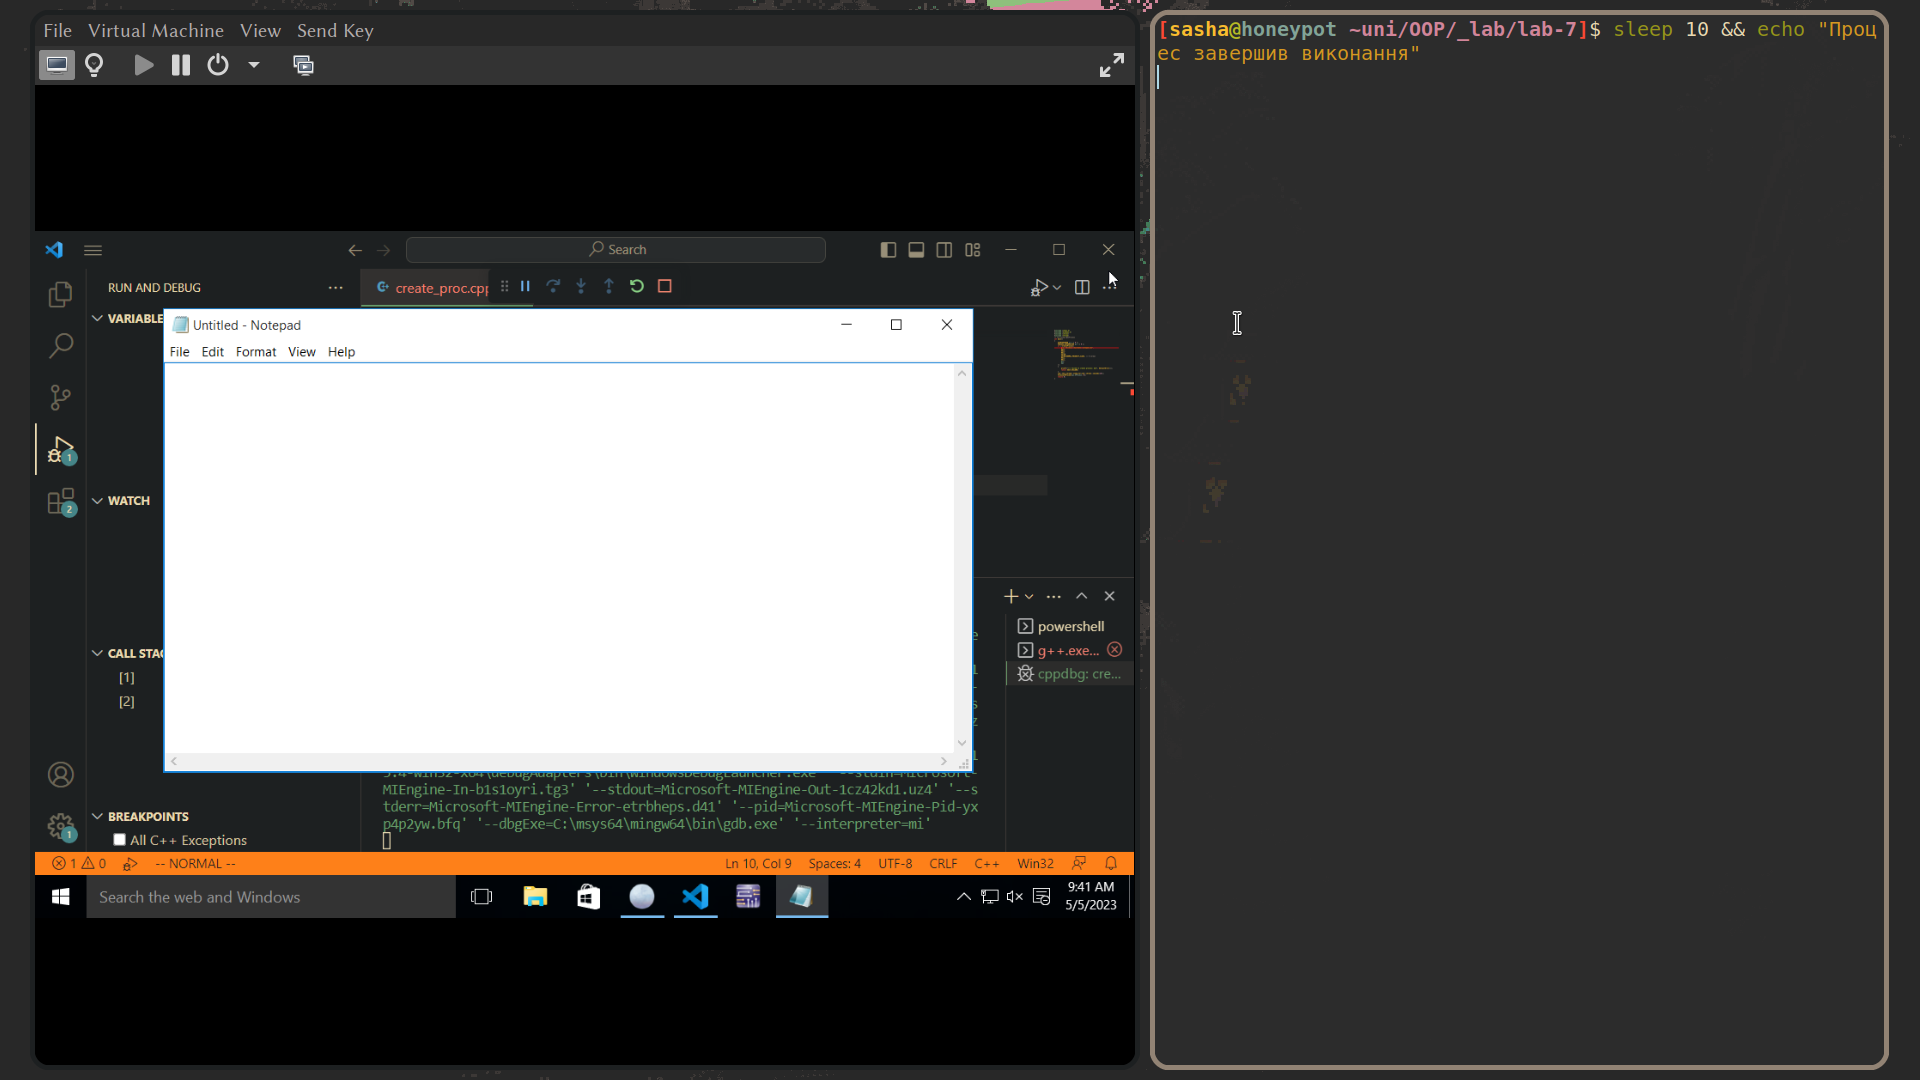
\includegraphics[width=\textwidth]{images/2}
	\caption{поява вікна програми}
\end{figure}
\begin{figure}[h]
	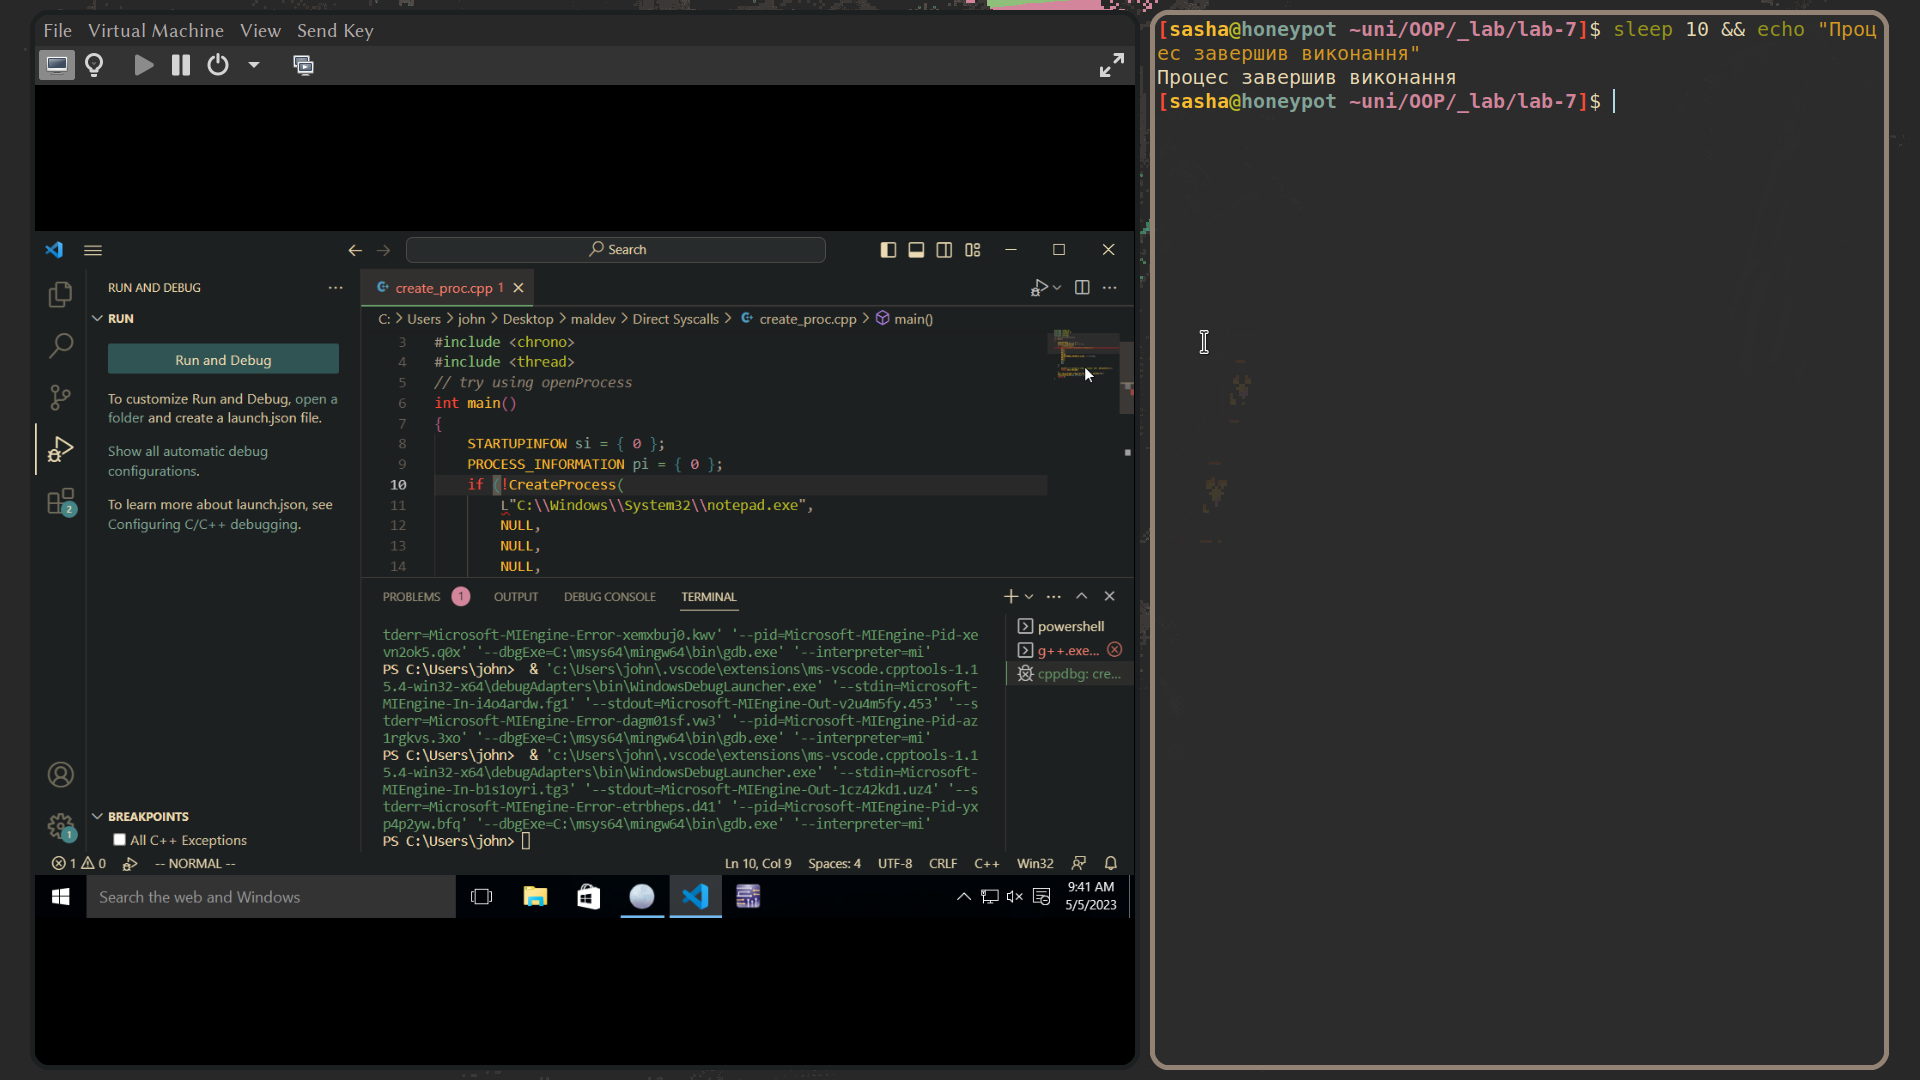
\includegraphics[width=\textwidth]{images/3}
	\caption{завершення}
\end{figure}
\clearpage

\paragraph{1.2}

\inputminted{c++}{1.2.cpp}
\subsection*{Результат виконання програми}
\inputminted{c++}{1.2.out}

\subsection*{завдання 2}
\inputminted{c++}{task_2.cpp}
\subsection*{Результат виконання програми}
\inputminted{c++}{task_2.out}

\subsection*{Результат виконання програми (стрічки з std::lock_guard закоментовані)}
\begin{verbatim}
locked by square_negativeslocked by non_negative_rows

-2^2
found4
found-5
-4^2
rows with no negative numbers: 1
1       4       3       16      5       6
1       2       3       4       5       6
1       2       3       4       -5      6
-5^2
1       4       3       16      5       6
1       2       3       4       5       6
1       2       3       4       25      6
\end{verbatim}

Бачимо, що без використання м'ютекса потоки працюють
із матрицею одночасно, що викликає невизначеність у
результатах.

\section*{Висновок}

У цій лабораторній роботі я навчився працювати з API Windows, запускати
процеси в різних потоках та синхронізувати їх.

\section*{Відповіді на контрольні запитання}
\begin{itemize}
	\question Що таке процес?
	\answer У комп'ютерних науках процес є екземпляром програми, який виконується на операційній системі і має власну адресний простір пам'яті, стек викликів, регістри та інші атрибути, що необхідні для його роботи.

	\question Яка АРІ-функція використовується для створення процесу?
	\answer Для створення процесу в операційній системі можна використати функцію API "CreateProcess" або її еквівалент у бібліотеці під назвою "fork" в UNIX-подібних операційних системах.

	\question Яка АРІ-функція використовується для завершення процесу?
	\answer Для завершення процесу в операційній системі можна використати функцію API "ExitProcess" або її еквівалент у бібліотеці під назвою "exit" в UNIX-подібних операційних системах.

	\question Що таке потік?
	\answer У комп'ютерних науках потік є послідовністю команд, яка виконується в межах процесу і має власний стек викликів та контекст виконання. Один процес може мати багато потоків, що дозволяє розділяти завдання між ними для досягнення кращої продуктивності.

	\question Що таке синхронізація потоків?
	\answer Синхронізація потоків - це механізм, який дозволяє контролювати порядок виконання потоків, щоб уникнути проблем, таких як гонка за даними (race conditions) і блокування (deadlocks). Взаємодія між потоками може відбуватися через спільну пам'ять або через передачу повідомлень.
	\question Види синхронізації:
	\answer
Виділяють 4 загальних типи синхронізації будь-яких двох потоків в одному процесі або будь-
яких двох процесів в одному додатку: старт-старт, фініш-старт, старт-фініш і фініш-фініш. За
допомогою цих базових типів відносин можна описати координацію завдань між потоками і
процесами.
		% \begin{itemize}
		% \item М’ютекс (mutex) - механізм, який дозволяє блокувати доступ до спільних ресурсів, щоб тільки один потік міг працювати з ними в один момент часу.
		% \item Семафор (semaphore) - механізм, який дозволяє обмежувати кількість потоків, що можуть доступатися до спільного ресурсу одночасно.
		% \item Умовна змінна
		% \item спін-блокування
		% \end{itemize}
	\question Які об’єкти використовуються для синхронізації потоків?
	\answer
		\begin{itemize}
			\item М’ютекс (mutex)
			\item Семафор (semaphore)
			\item подія (event)
		\end{itemize}
	\question Що таке об’єкт синхронізації «подія»?
	\answer Подією називається сповіщення про деяку виконану дію. У програмуванні
події використовуються для сповіщення одного потоку про те, що інший потік
виконав деяку дію. Такі задачі відносяться до задач умовної синхронізації. У
операційних системах Windows події описуються об'єктами ядра Events.
\end{itemize}

\end{document}
